\documentclass{article}
\usepackage[utf8]{inputenc}
\usepackage{float}
\usepackage{xcolor}
\usepackage{graphicx}
\usepackage{amsmath}
\usepackage{amssymb}
\usepackage{placeins}
\usepackage{booktabs}
\usepackage{caption}

\usepackage{hyperref}
\hypersetup{
    colorlinks=true,
    linkcolor=blue,
    filecolor=magenta,      
    urlcolor=blue,
}

\title{Scientific Computing - Molecular dynamics \\ Group F}
\newcommand{\subtitle}{Problem sheet 3}
\author{
    Jimin Kim \\
    Christian Nix \\
    Noah Schlenker
}
\date{\today}

\begin{document}

\maketitle

\begin{center}
    \LARGE \subtitle{}
\end{center}

\section{Pull request}
\label{sec:pr}
The pull request can be found \href{https://github.com/noahpy/MolSim-SS24/pull/33}{here}.

\section{XML format adaptation}
\label{sec:xml}

\begin{itemize}
    \item We defined the structure and constraints for XML files using XSD .
    \item The key elements specified include:
    \begin{itemize}
        \item Standard parameters as outlined in Task 1, such as base name and cuboid specification etc.
        \item Domain specifications and cutoff-radius
        \item Boundary condition specifications
    \end{itemize}
    \item The directory containing generated C++ code, enabling XML parsing, is added to the include path for our target \texttt{src}
    \item We utilized several flags in the XSD CMake module:
    \begin{itemize}
        \item \texttt{cxx-tree}: Converts XML documents to a tree-like in-memory object model, generating corresponding C++ classes.
        \item \texttt{--hxx-suffix=.h} and \texttt{--cxx-suffix=.cpp}: Specifies suffixes for the generated header and source files.
        \item \texttt{--std=c++11}: Ensures the generated C++ code adheres to the C++11 standard.
        \item \texttt{--generate-doxygen}: Adds Doxygen comments to the generated code.
        \item \texttt{--generate-serialization}: Includes serialization support, allowing XML data to be read from and written to XML documents.
    \end{itemize}
\end{itemize}

\section{Linked-Cell Algorithm}
\label{sec:lc}

\begin{itemize}
    \item We added the cell and cell-grid to the models to implement the linked-cell algorithm (see \texttt{src/models/linked\_cell}).
    \item A new simulation class \texttt{linkedLennardJonesSim} and force calculation function \texttt{force\_lennard\_jones\_lc} were introduced for using linked-cells in our project structure (see \texttt{src/simulation} and \texttt{src/physics/forceCal}).
    \item Each added section has its corresponding Unit tests.
\end{itemize}

\subsection{Cells}
\label{subsec:cell}

\begin{itemize}
    \item Each cell contains a list of references to particles and a \texttt{type} attribute, categorized as \texttt{inner}, \texttt{boundary}, or \texttt{halo}.
    \item The \texttt{CellIndex} and \texttt{neighborCounter} attributes are essential for the cell-grid structure.
    \item Neighbor vectors include information on the index and position of boundary, inner, and halo neighbors within the grid.
    \item A \texttt{PairListIterator} enables iteration over unique pairs in the reference list.
\end{itemize}

\subsection{Cell Grid}
\label{subsec:grid}

\begin{itemize}
    \item Our cell grid is implemented using a 3-dimensional vector matrix, \texttt{CellVec}, which contains \texttt{std::unique\_ptr} to cells.
    \item Initialization requires \texttt{domainSize}, \texttt{domainOrigin}, and \texttt{cutoffRadius}, and performs the correct cell type selection.
    \item The initialization function ensures uniform and fitting cell sizes.
    \item Particle references in each cell's list are assigned from the existing particle container's vector.
    \item This file includes most necessary functions for running a simulation and calculating forces using the linked-cell algorithm.
    \item Noteworthy is the function \texttt{std::list<CellIndex> getNeighbourCells(const CellIndex\& cellIndex) const}, which returns a list of neighboring cell indices for a given cell:
    \begin{itemize}
        \item We needed an algorithm to utilize newton's third law on cell iteration level.
        \item Similar to the unique pair iteration on the lists in cells, we implemented a method to distinguish between neighbor pairs, that already have been calculated.
        \item Given an index to a cell, our function iterates over each neighboring cell and increments the parameter cell's \texttt{neighborCounter} for each non-halo neighbor.
        \item If a neighboring cell's \texttt{neighborCounter} is greater than 0, its counter is decreased, and the neighbor is ignored.
        \item Otherwise, the neighbor's index is added to the return list.
        \item The usage of simple increment and decrement operations ensure an efficient way to improve cell iteration and keep calculations to a minimum. The speedup of our linked-cell implementation is showcased in section\ \ref{subsec:perflc}.
    \end{itemize}
    \item We implemented the iterators for halo and boundary cells in a separate file for clarity.
    \item We extended the UML diagram for visualization of the new project structure as seen here\ \ref{fig:uml}. The added UML section ties into our previous UML diagram through the connection seen in\ \ref{fig:uml2}.
\end{itemize}

\begin{figure}[H]
    \centering
    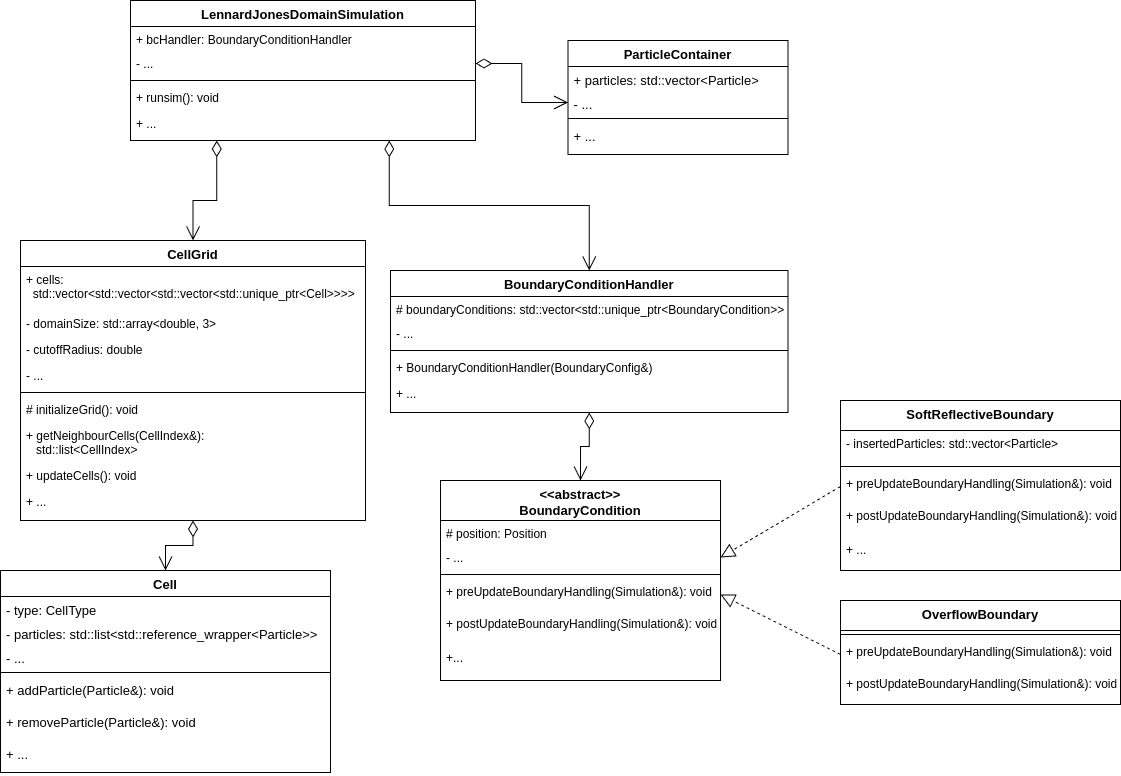
\includegraphics[width=0.9\textwidth]{res/UML3.drawio}
    \caption{UML diagram extension.}
    \label{fig:uml}
\end{figure}

\begin{figure}[H]
    \centering
    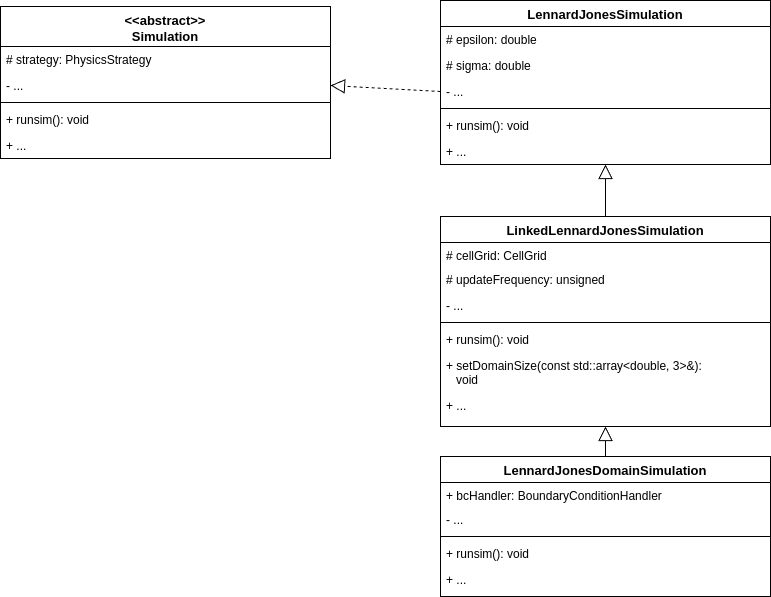
\includegraphics[width=0.6\textwidth]{res/UMLSimulation3.drawio}
    \caption{Connection of the extended UML part and the overall UML diagram structure through abstract class Simulation.}
    \label{fig:uml2}
\end{figure}

\subsection{Performance test}
\label{subsec:perflc}

\begin{itemize}
    \item We added a benchmark test for the linked-cell implementation \newline(see \texttt{bench/benchLinkedCell.cpp}).
    \item The performance was tested with the parameters stated in Task 2 and compared with our naive Lennard-Jones simulation.
    \item The hardware specifics for running the tests are the same as last assignment.
    \item The data collected can be seen below. Google benchmark provided a runtime analysis stated in Big O-notation.\newline
    \newline
    \begin{tabular}{|c|c|c|c|}
        \toprule
        Benchmark/\#Particles & Time & CPU & Iterations \\
        \toprule
        BM\_LJSimulation/1000 & 1.4485e+10 ns & 1.4477e+10 ns & 1 \\
        \midrule
        BM\_LJSimulation/2000 & 5.7983e+10 ns & 5.7959e+10 ns & 1 \\
        \midrule
        BM\_LJSimulation/4000 & 2.3180e+11 ns & 2.3171e+11 ns & 1 \\
        \midrule
        BM\_LJSimulation/8000 & 9.2722e+11 ns & 9.2686e+11 ns & 1 \\
        \midrule
        BM\_LJSimulation\_BigO & 14487.81 $N^2$ & 14482.20 $N^2$ & - \\
        \midrule
        BM\_LinkedLJSimulation/1000 & 28515871 ns & 28493193 ns & 25 \\
        \midrule
        BM\_LinkedLJSimulation/2000 & 54951418 ns & 54934137 ns & 13 \\
        \midrule
        BM\_LinkedLJSimulation/4000 & 114455900 ns & 114424760 ns & 6 \\
        \midrule
        BM\_LinkedLJSimulation/8000 & 236827726 ns & 236733811 ns & 3 \\
        \midrule
        BM\_LinkedLJSimulation\_BigO & 29304.28 $N$ & 29293.31 $N$ & - \\
        \bottomrule
    \end{tabular}
    \item We can observe an improvement from squared to linear runtime!
    \item A graphical representation with additional particle numbers are shown in\ \ref{fig:timelc} and\ \ref{fig:timelclong}.
\end{itemize}

\FloatBarrier

\begin{figure}[H]
    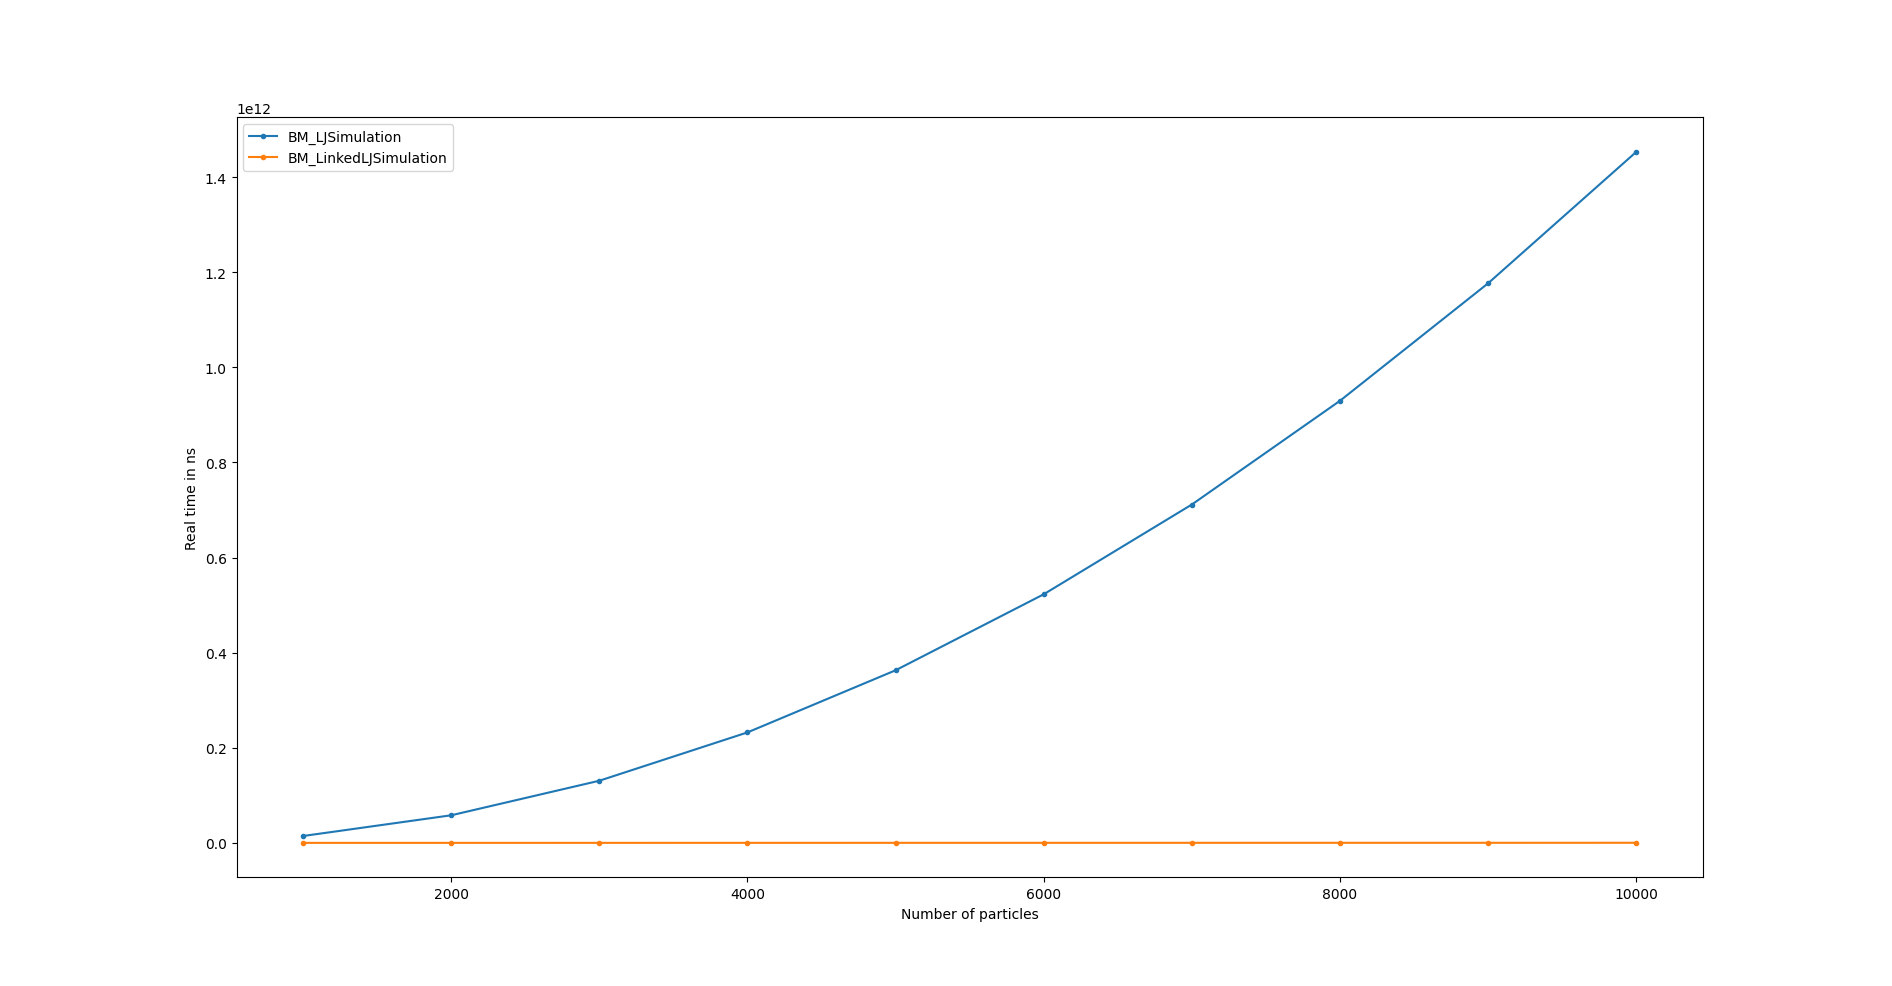
\includegraphics[width=\textwidth]{res/lj_big_plot_linear}
    \caption{linked-cell and naive simulation times of a 2D-square with 1000 to 10000 molecules.}
    \label{fig:timelc}
\end{figure}

\begin{figure}[H]
    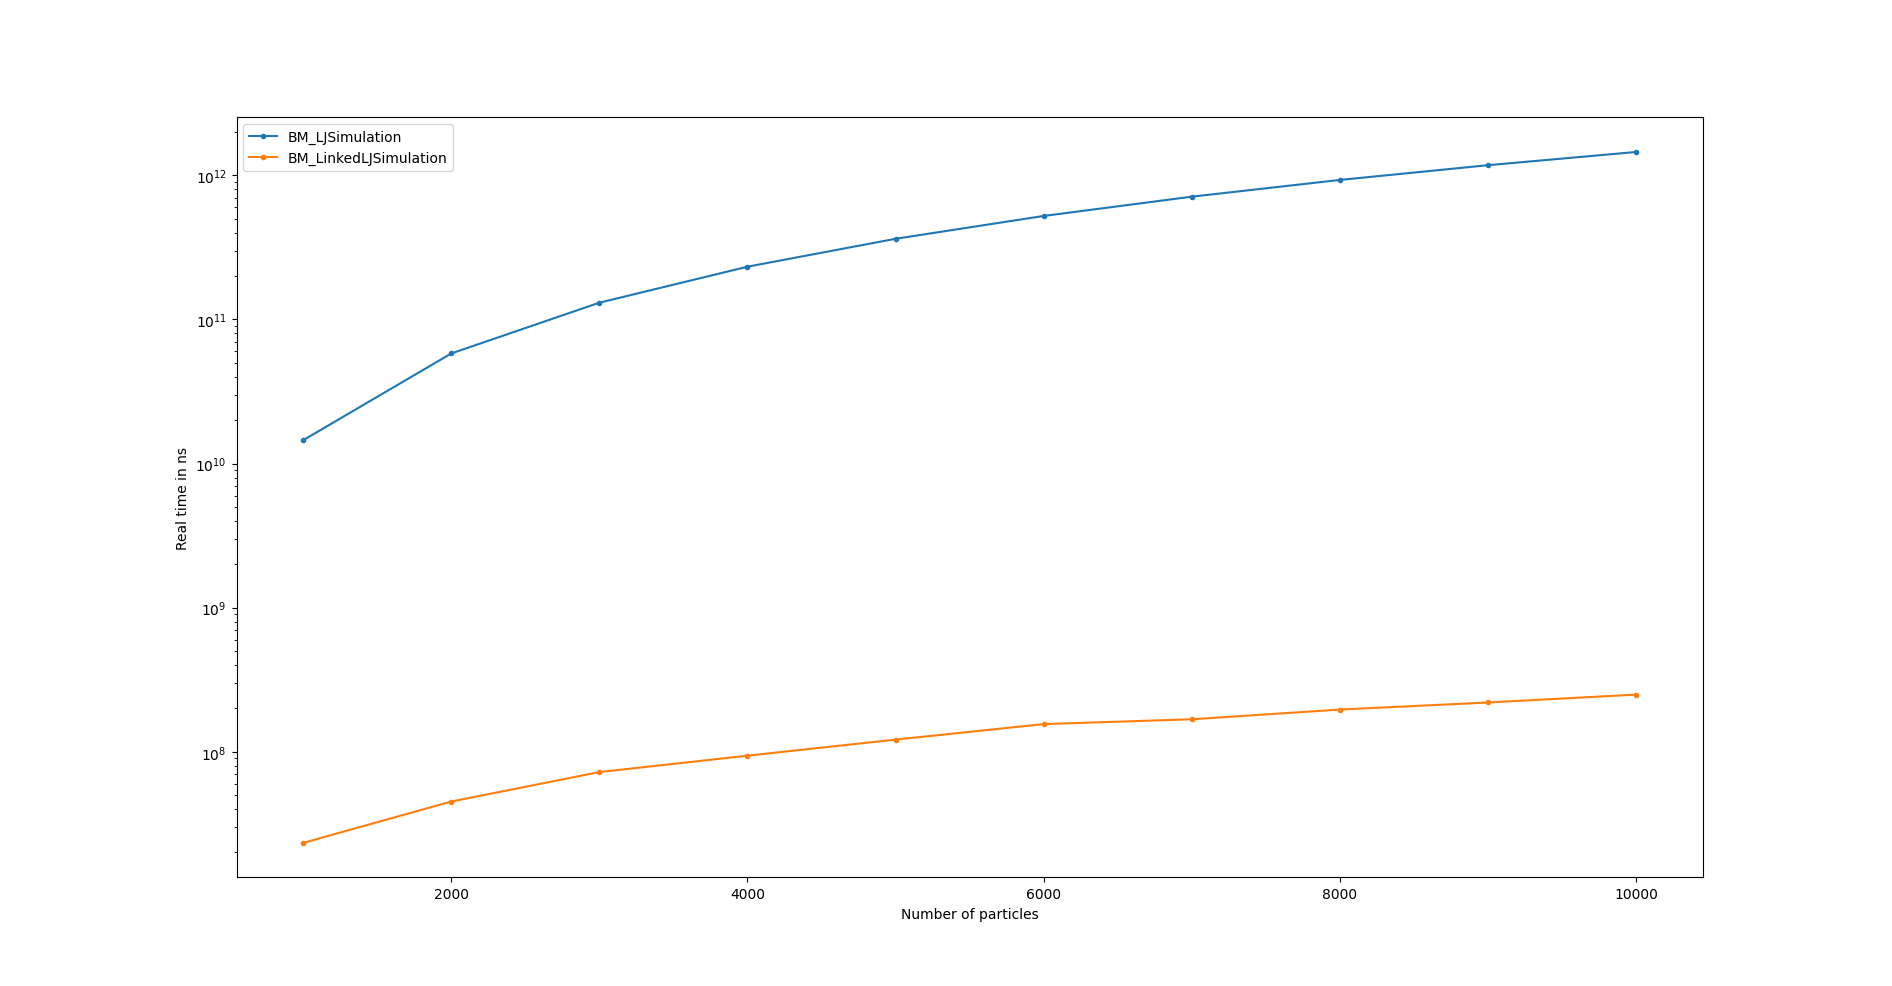
\includegraphics[width=\textwidth]{res/lj_big_plot_log}
    \caption{linked-cell and naive simulation times with 1000 to 10000 particles on a logarithmic time scale}
    \label{fig:timelclong}
\end{figure}

\section{Boundary Conditions}
\label{sec:bound}

\begin{itemize}
    \item We added boundary conditions to the physics section of our project (see \texttt{src/physics/boundaryConditions}).
    \item A Handler organizes the conditions for each boundary in a simulation specified in the boundary configuration file.
    \item The boundary condition is a virtual class, and provides functions for applying the conditions before and after updates in the cell grid.
    \item We have two implementations of boundary conditions as described in the third meeting:
    \begin{itemize}
        \item \texttt{OverflowBoundary}: Particles, that would leave the domain, get stuck at boundaries and are considered removed, as they no longer take part in any calculations. We will provide a deletion of the particles from the actual particle vector in the future by changing the references to particles in cells to shared pointers.
        \item \texttt{SoftReflectiveBoundary}: Particles are reflected from the boundaries via a mirrored ghost particle in the neighboring halo cell. This required an additional function to find the relevant halo cell for creating the ghost particle.
    \end{itemize}
\end{itemize}

\section{Sphere generation}
\label{sec:sphere}

\begin{itemize}
    \item We extended the particle generators with a class to generate sphere clusters (see \texttt{src/models/generators/SphereParticleCluster})
    \item The logic of sphere generation can be split into 2D and 3D:
    \begin{itemize}
        \item 2D Discs: The disc is created as a collection of concentric rings of particles. A ring is generated with particles evenly spaced around a circumference. Then rings with decreasing radii are accumulated to form a disc.
        \item 3D Sphere: The sphere is constructed as a stack of discs. Discs above and below the origin are iteratively generated with decreasing radii.
    \end{itemize}
    \item Our generated sphere can be seen here\ \ref{fig:sphere}.
    \item We achieve even spacing of particles in rings through the use of several trigonometric functions:
    \begin{enumerate}
        \item Angular step calculation:
        \begin{itemize}
            \item We calculate the angular step $\theta$ between particles to ensure they are spaced by at least a given distance along the circumference.
            \item Given a ring with radius \textit{r} and particle spacing \textit{s}, the angular step $\theta$ is determined by:
            \item $\theta = 2 \arcsin\left(\frac{s}{2 \times r}\right)$
        \end{itemize}
        \item Number of particles calculation:
        \begin{itemize}
            \item The number of particles \textit{N} that can fit in the ring is given by dividing the full circle ($2\pi\ radians$) by the angular step $\theta$:
            \item $N = \left\lfloor \frac{2\pi}{\theta} \right\rfloor$
        \end{itemize}
        \item Positioning particles:
        \begin{itemize}
            \item The coordinates for each particle in the ring are calculated using polar coordinates.
            \item For a particle at index \textit{i}, the position is:
            \item $x_i = \text{origin}_x + r \cos(i \theta)\newline y_i = \text{origin}_y + r \sin(i \theta)\newline z_i = \text{origin}_z + \text{z\_offset}$
        \end{itemize}
    \end{enumerate}
\end{itemize}

\begin{figure}[H]
    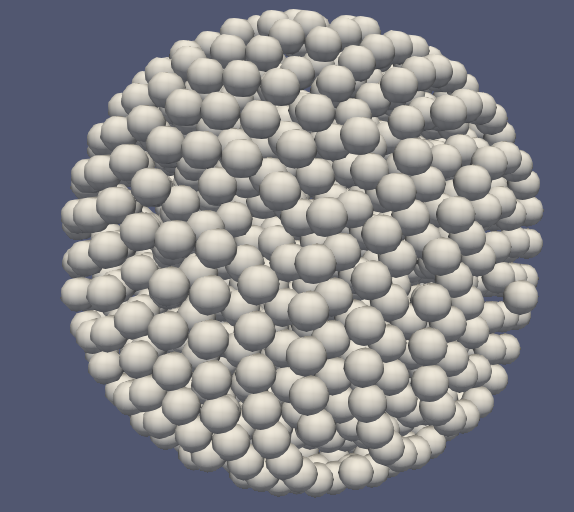
\includegraphics[width=\textwidth]{res/sphere}
    \caption{A sphere created by our generation algorithm}
    \label{fig:sphere}
\end{figure}

\end{document}
